% =====================================================================
% A28 — Supplementary main-result figures relocated from the body to meet the
% ICLR 9-page main-text limit. Both figures are referenced from the main text
% (\cref{sec:decision-surface}, \cref{sec:exp-sota}); labels are unchanged so all
% main-text \cref / \ref calls resolve here. Figures and numbers are identical to
% the body version (verifier-checked, no re-computation). caveman OFF.
% =====================================================================

\section{Supplementary Main-Result Figures and Tables}\label{app:moved-figs}
To respect the nine-page main-text limit, two result figures and the SOTA-comparison table referenced
in the main text are reproduced here in full resolution: the reliability\,$\times$\,recoverability
decision surface of \cref{sec:decision-surface}, the enhancement-versus-restoration comparison of
\cref{sec:exp-sota}, and the E10 generic-restoration table (\cref{tab:e10}). The accompanying numbers
are stated in the main text and in Appendix~\ref{app:a2-prop3} and the cost-benefit appendix; nothing
here is recomputed.

% E10 --- QP-Enhance vs 6 generic non-diffusion restoration SOTA (zero-shot).
% Frozen 会话28: job 1448952 (stored-mixed 降质, n=10881 paired, 117 melanoma; 与 E1 同
% degrade 算子 -> QP-Enhance PSNR 32.79 == E1 32.74 caliber). 数字 csv: results/e10_<m>.csv.
% 会话43 富表升级（BMVC 风格）: 彩色阴影 + per-column 粗体最优/下划线次优 + paired CI 列。
%   所有数字逐字搬自 STORY 锁定值 / ACCEPTANCE C1.4（results/e10_*.csv，verifier 核），零重算。
%   诚实红线（STORY L248 / ACCEPTANCE L183 dflip 单指标陷阱）：QP-Enhance dflip 0.194
%   非最优，绝不标粗/不标赢；dflip 列粗体给 Uformer 0.054（最优）、下划线给 Restormer 0.059。
% caveman OFF.
\begin{table}[!ht]
\centering
\caption{\textbf{E10 --- diagnosis preservation versus six generic restoration SOTA, zero-shot.}
All methods restore the identical mixed-severity degraded inputs, $n{=}10{,}881$ paired with $117$
melanomas. \textbf{Bold}/\underline{underline}: best/second per column; green: where \visienhance{}
wins. \visienhance{} wins five of six metrics, and every baseline is a significantly worse diagnostic
preserver: the paired block reports all $95\%$ CIs excluding $0$ with McNemar $p<10^{-150}$.
It does \emph{not} win dflip; actively rewriting within the salvage band occasionally flips a
melanoma, the motivation for query-for-retake (\cref{sec:agent}). The lowest-dflip baselines are also
the blurriest, with the highest KL and lowest consistency.}
\label{tab:e10}
\footnotesize
\setlength{\tabcolsep}{4.5pt}
\renewcommand{\arraystretch}{1.05}
\begin{tabular}{l l c c c c c c}
\toprule
Method & Pretraining & PSNR\,$\uparrow$ & SSIM\,$\uparrow$ & $\Delta$AUC\,$\to0$ & Consist.\,$\uparrow$ & KL\,$\downarrow$ & dflip\,$\downarrow$ \\
\midrule
\rowcolor{green!12}\textbf{\visienhance{} (FiLM+DP)} & dermoscopy
 & \cellcolor{green!18}\textbf{32.79}
 & \cellcolor{green!18}\textbf{0.907}
 & \cellcolor{green!18}\textbf{$-$0.017}
 & \cellcolor{green!18}\textbf{0.955}
 & \cellcolor{green!18}\textbf{0.10}
 & 0.194 \\
\midrule
Restormer \citep{zamir2022restormer}   & real denoising  & 22.30 & 0.836 & \cellcolor{red!16}$-$0.096 & 0.684 & 0.82 & \underline{0.059} \\
NAFNet \citep{chen2022simple}          & SIDD denoising  & 22.04 & 0.825 & \cellcolor{red!20}$-$0.115 & 0.669 & 0.88 & 0.077 \\
MIRNet-v2 \citep{zamir2022mirnetv2}    & LOL enhancement & 13.48 & 0.775 & \cellcolor{red!14}$-$0.087 & 0.818 & 0.50 & 0.158 \\
SwinIR \citep{liang2021swinir}         & colour denoising& 21.69 & 0.786 & \cellcolor{red!22}$-$0.134 & 0.821 & 0.36 & 0.478 \\
Uformer-B \citep{wang2022uformer}      & SIDD denoising  & 22.28 & \underline{0.836} & \cellcolor{red!16}$-$0.094 & 0.683 & 0.83 & \textbf{0.054} \\
Real-ESRGAN \citep{wang2021realesrgan} & $\times2$ SR    & 21.61 & 0.818 & \cellcolor{red!12}\underline{$-$0.083} & \underline{0.851} & \underline{0.35} & 0.234 \\
\midrule
\multicolumn{8}{l}{\textit{Paired $\Delta\mathrm{AUC}_{\text{baseline}-\text{VE}}$ vs.\ \visienhance{} (negative = baseline worse; $95\%$ CI; all exclude $0$):}}\\
\multicolumn{8}{l}{\;\; Restormer $-0.079\,[-0.096,-0.064]$\quad NAFNet $-0.098\,[-0.116,-0.080]$\quad MIRNet-v2 $-0.070\,[-0.088,-0.054]$}\\
\multicolumn{8}{l}{\;\; SwinIR $-0.116\,[-0.135,-0.098]$\quad Uformer-B $-0.077\,[-0.093,-0.061]$\quad Real-ESRGAN $-0.066\,[-0.082,-0.050]$}\\
\bottomrule
\end{tabular}
\end{table}


% Fig: composite decision surface. (A) reliability AUC curves; (B) recoverability heatmap.
\begin{figure}[t]
\centering
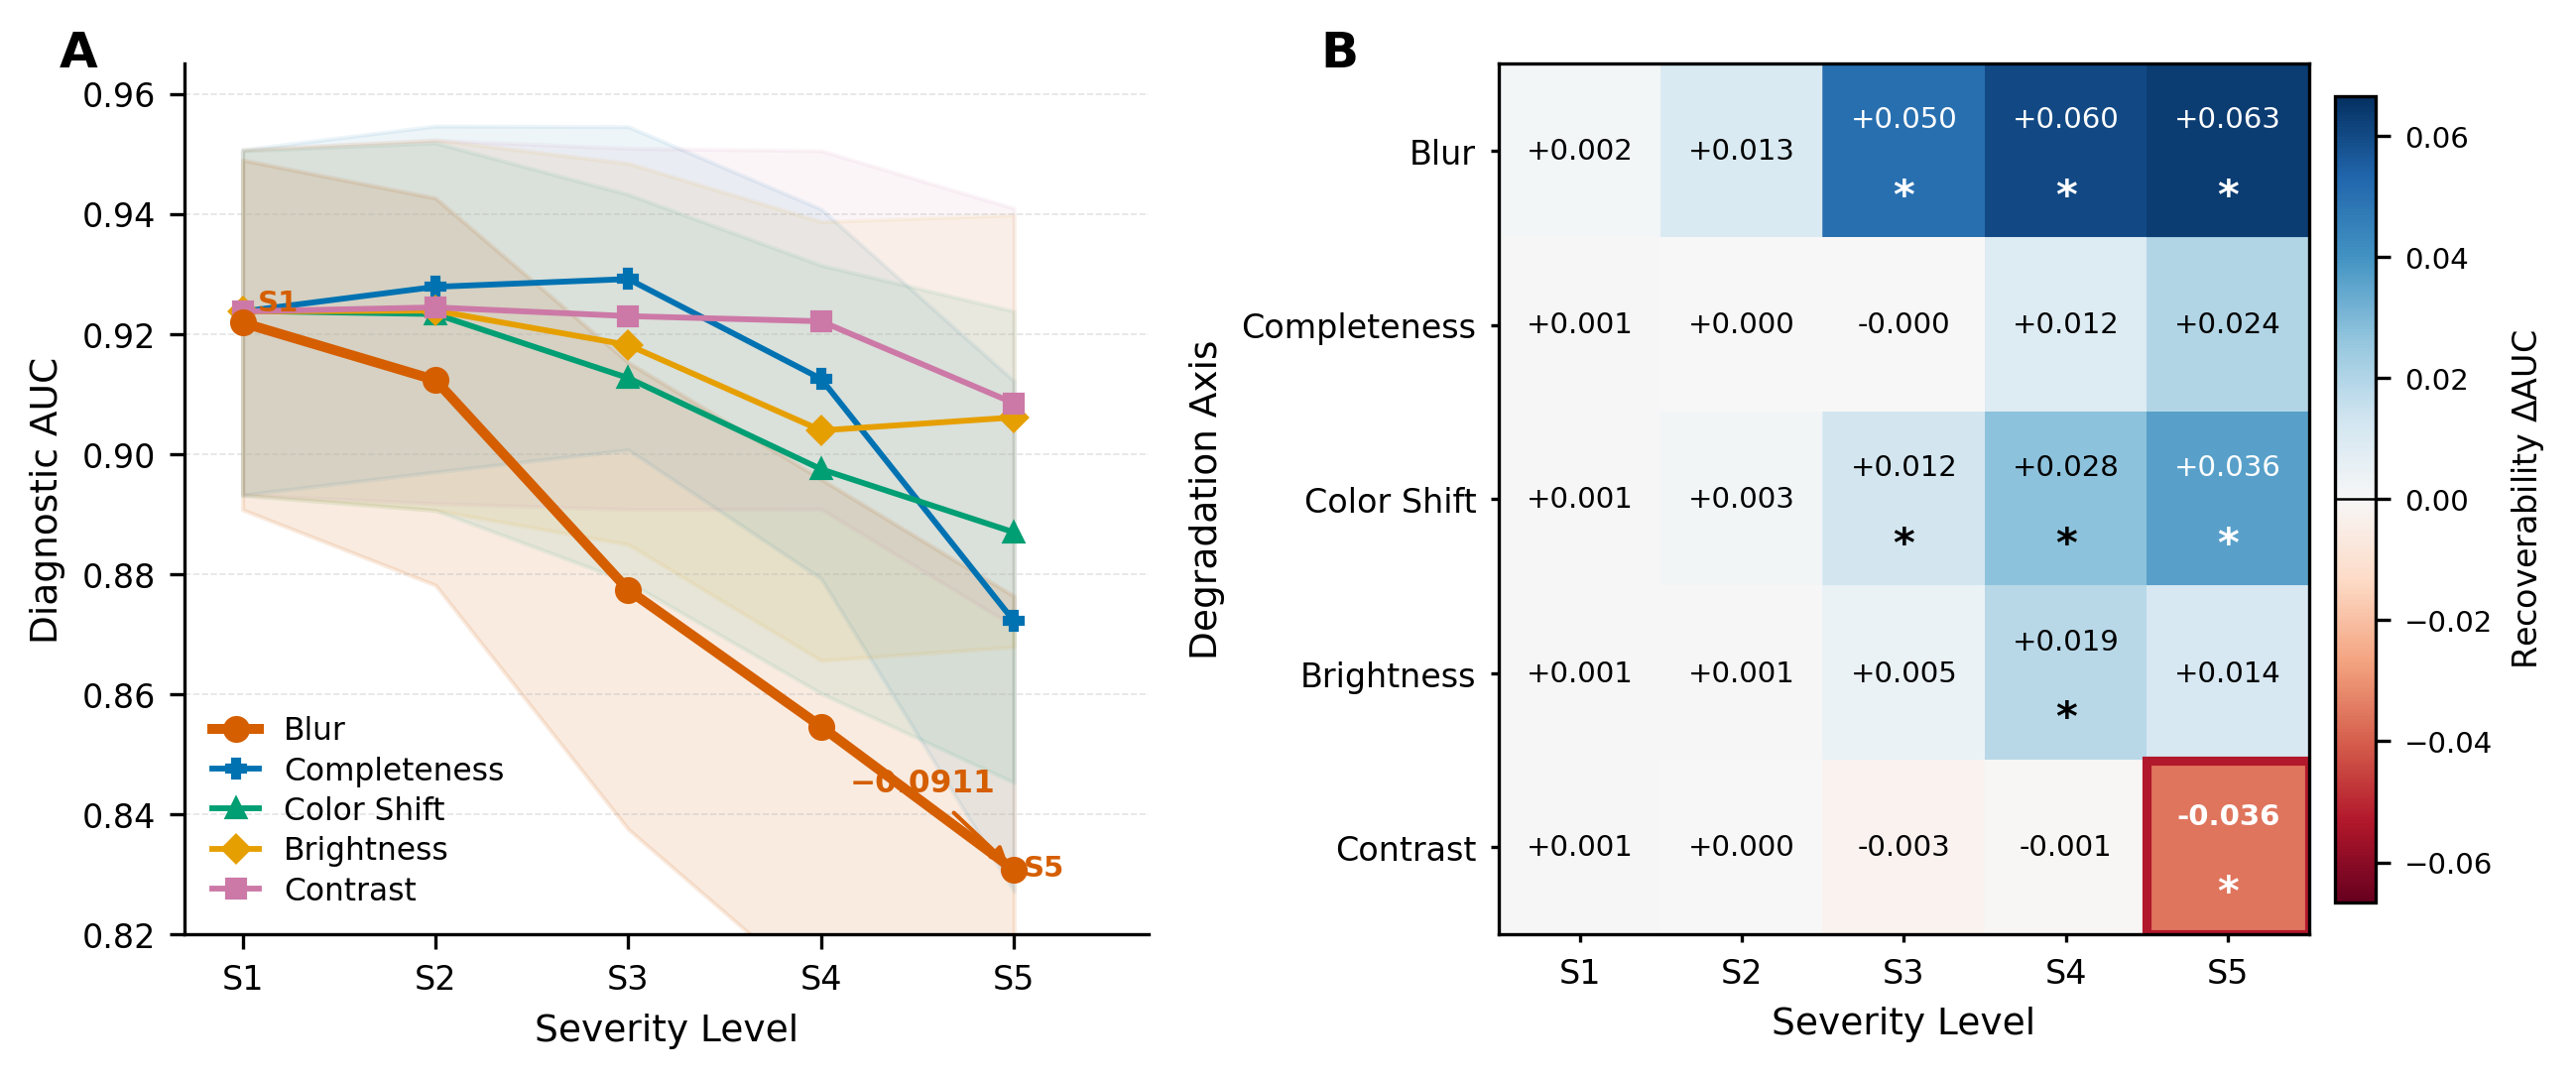
\includegraphics[width=0.85\linewidth]{figures/fig2_decision_surface.pdf}
\caption{\textbf{Reliability~$\times$~recoverability decision surface} over the five-dimension $\times$ five-severity grid ($n=360$/cell). \textbf{(A)} Diagnostic AUC declines monotonically with severity; blur is by far the most fragile dimension ($\Delta=-0.0911$ from S1 to S5). \textbf{(B)} Recoverability $\Delta=\mathrm{AUC}_{\mathrm{enh}}-\mathrm{AUC}$ per cell (diverging scale; starred cells have a bootstrap $95\%$ CI excluding zero): enhancement helps across the moderate window but significantly hurts exactly one of $25$ cells, contrast at S5. Full per-cell values and CIs in Appendix~A5\_2.}
\label{fig:c0-surface}
\end{figure}

\begin{figure}[t]
  \centering
  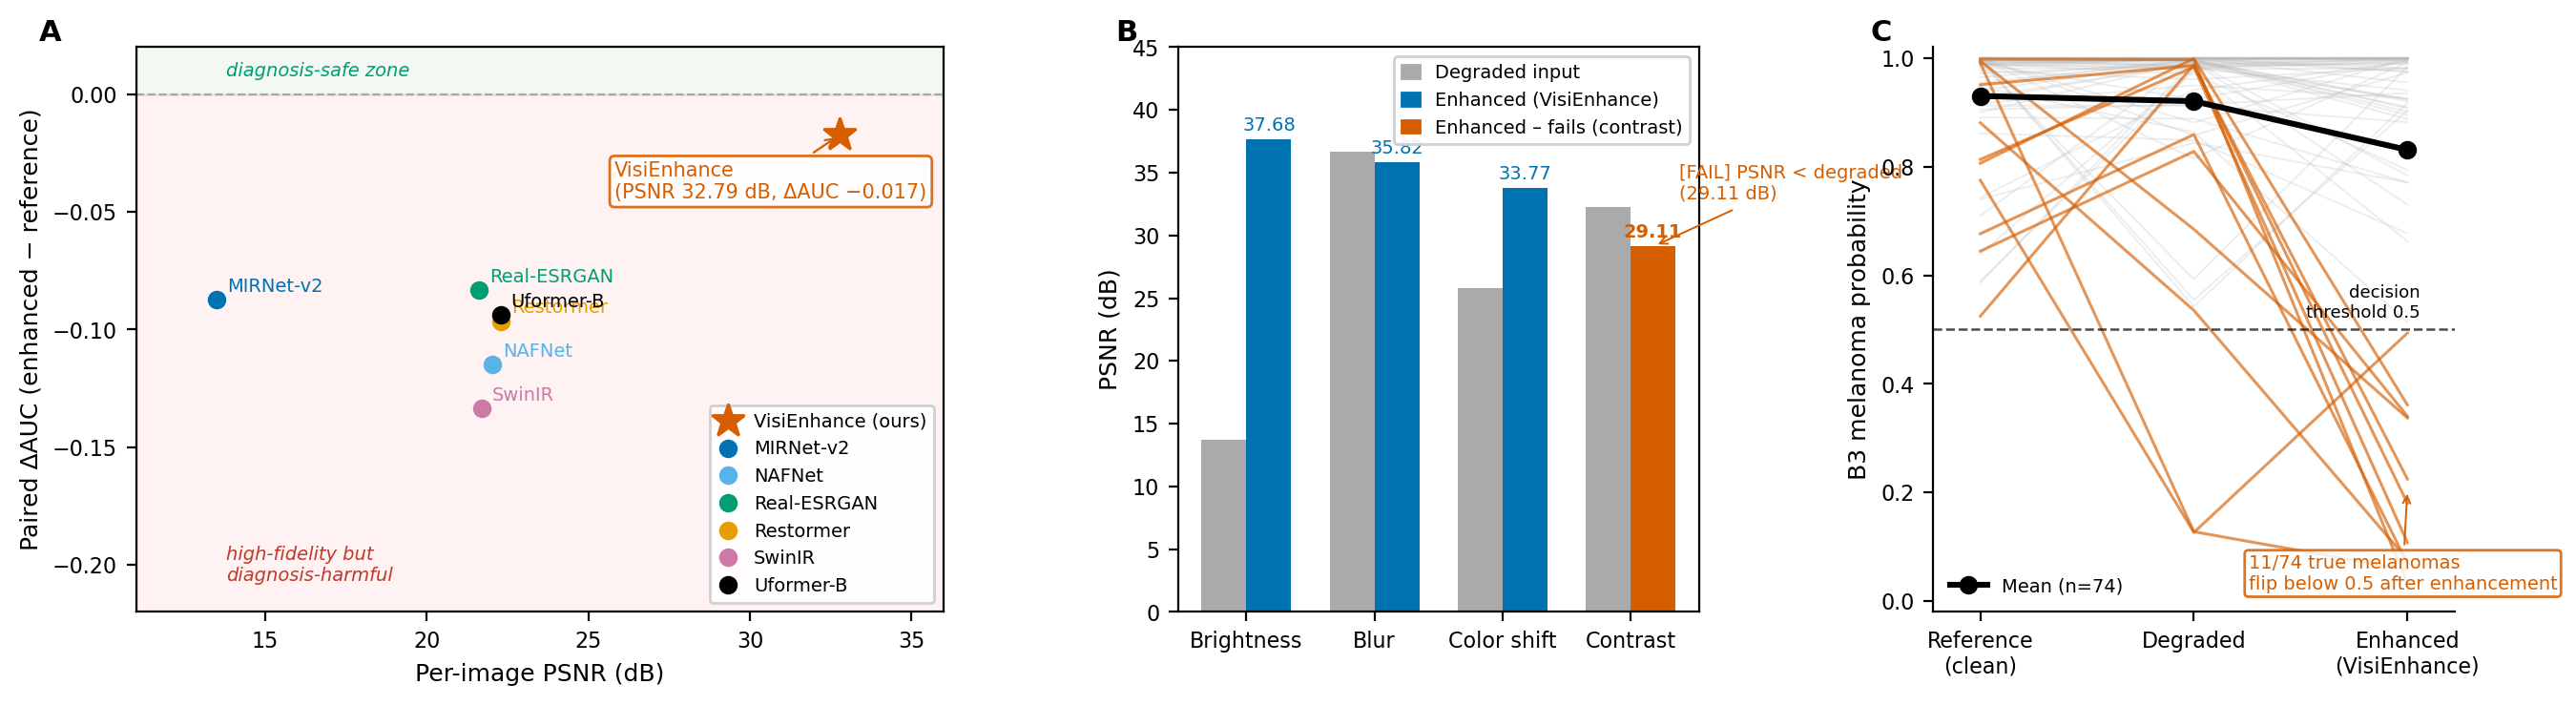
\includegraphics[width=0.85\linewidth]{figures/fig3_enhancement.pdf}
  \caption{\textbf{Diagnosis-preserving enhancement versus generic restoration.}
  \textbf{(A)} Fidelity\,/\,diagnosis-preservation trade-off: each point is one zero-shot
  restoration model on identical mixed-severity degraded inputs ($n{=}10{,}881$ paired,
  $117$ melanomas); \visienhance{} is the only model in the safe corner (high PSNR,
  $\Delta\mathrm{AUC}\!\approx\!0$), whereas generic restorers sacrifice fidelity or
  diagnostic preservation. \textbf{(B)} Per-dimension restoration PSNR: enhancement helps
  brightness and blur but is harmful on contrast ($29.11$\,dB, below the degraded input's
  own $32.29$\,dB). \textbf{(C)} Residual \emph{dangerous flips}: enhancement still pushes a
  small subset of correctly-called melanomas below the decision threshold (sources
  \texttt{results/e10\_*.csv}, \texttt{e2\_perdim.csv}, \texttt{dflip\_persample\_v6.csv}).}
  \label{fig:enhancement}
\end{figure}
